\documentclass[titlepage, 11pt]{article}
\renewcommand{\refname}{9 \ \ WORKS CITED}
\usepackage[margin=0.5in]{geometry}
\usepackage{amsmath}
\usepackage{amssymb}
\usepackage{bm}

\usepackage{graphicx,caption,threeparttable}
\graphicspath{ {images/} }

\begin{document}

\title{Sketch-based Model Fracturing}
\author{
Alfonso Mu\~{n}oz\\
Andrew Heng\\
Duc Daniel Do\\
[1cm]{\small Instructor:}\\
\small{Dr. Faramarz Samavati}
}
\maketitle

\section{ABSTRACT}
In this project, we propose the creation of a sketch based system for the production of fractured versions of existing 3D models. This will be done by extending the procedural fracturing methodology introduced by Van Gestel et al. to make use of sketch-based input. Such a system could aid in the game and film production process by allowing artists to generate fractured versions of models without having to recreate them.

\section{INTRODUCTION}
There is an ever increasing demand for high fidelity meshes to be used in media like film and games. The rising cost associated with this demand is often mitigated by taking a procedural approach to content generation. Procedural approaches like model fracturing as proposed by Van Gestel et al.$^{[1]}$, allow for faster content generation by modifying existing content with effects controlled by different parameters. This reduces the need to create different variations of the same objects to meet the differing criteria. However, artists have limited control over the results of procedurally generated models. We propose that the introduction of a sketch-based approach to model fracturing would allow artists to have interactive control over procedural content generation.

\section{GOALS AND OBJECTIVES}
The goal of this project is to create a proof of concept of a system that would allow users to define fractures on existing models using a sketch-based approach and to be able to export the resulting meshes in media like film or games.\\
\\In order to accomplish our goal, we have outlined several objectives that we are to meet:
% 3.1
\subsection{Model Viewer}
Our system must allow the user to be able to view and interact with 3D meshes. The system must also support importing and exporting meshes.
% 3.2
\subsection{Sketch-based Input}
Our system must have an effective methodology for sketch-based user input.
% 3.3
\subsection{Fracture Objects}
Our system will support the fracturing of 2D and 3D meshes via sketching and allow exporting of fractured meshes for use in other media.
% 3.4
\subsection{Further Enhancements}
If time permits, we would like to improve upon the UX design and controls of the system, be able to support more file formats, and add support for texture fracturing.
% Methodology
\section{METHODOLOGY}
\subsection{User Sketching}
Our interface will allow the user to generate a collection of control points that will create a B-Spline curve of user-defined order.
\subsection{Fracture Mesh}
The B-Spline curve from the user sketch will define the fracture pattern for the object. The fracture pattern will then be transformed into a 3D plane. We can then generate the mesh of the fracture by extruding the cross-section definition in a direction perpendicular to the original mesh (see Figure 1). To do so, we will explore plane/line intersections with 3D objects.
\begin{figure}
\begin{center}
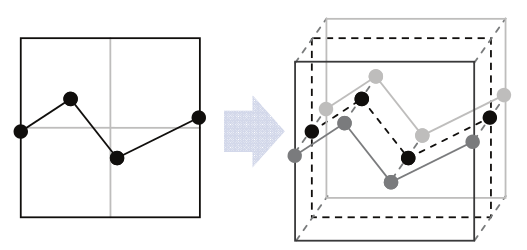
\includegraphics[scale=0.4]{fracture_pattern.png}
\caption{Fracture pattern extruded to a three dimensional fracture mesh.$^{[1]}$}
\end{center}
\end{figure}

\section{EXPECTED RESULTS}
The creation of the system may aid in the content generation process by allowing artists to produce higher quality fractured objects through sketching.

\section{TIMELINE}
{[Objective 1]} Model Viewer - done approx. February 17\\
{[Objective 2]} Sketch based Input - done approx. February 24\\
{[Objective 3.a]} Fracturing 2D Objects - done approx. March 10\\
{[Objective 3.b]} Fracturing 3D Objects - approx. March 24

\section{TECHNOLOGIES}
C++, OpenGL, GLM, AssImp

\section{GROUP RESPONSIBILITY}
Individual responsibility will be determined on a weekly basis. This would be dependent on the project status and what is required. 

\begin{thebibliography}{1}

\bibitem{objfrac} Van Gestel, J \& Bidarra, Rafael. (2011). {\em Procedural Modelling of Destructible Materials}.

\end{thebibliography}

\end{document}